\documentclass{beamer}
 
\usepackage[utf8]{inputenc}

\usetheme{Copenhagen}
 
\makeatletter
\newcommand\mysphere{%
  \parbox[t]{10pt}{\raisebox{0.2pt}{\beamer@usesphere{item projected}{bigsphere}}}}
\makeatother

%Information to be included in the title page:
\title[Learning with your spouse] %optional
{Learning with your spouse: Does the similarity of spouse's occupation affect individual's earning?}
 
\subtitle{}
 
\author[Ningyin, Xu] % (optional, for multiple authors)
{Ningyin Xu}
 
\institute[University of Chicago] % (optional)
{MACSS, University of Chicago}
 
\date[4/5/2017] % (optional)
{April 5th, 2017}
 
\begin{document}

\frame{\titlepage}
 
\begin{frame}
\frametitle{Table of Contents}
\tableofcontents
\end{frame}

\section{Research Question} 
\begin{frame}
\frametitle{Research Question}
To what extent the occupational similarity between one's partner and herself/himself would influence one's income?
\begin{block}{Hypothesis}
Controlling one's education-level, age, sex, and occupation, I expect with higher similarity of spouse's occupation, one's after-marriage income would be relatively higher.
\end{block}
\end{frame}

\section{Literature Review} 
\begin{frame}
\frametitle{Literature Review}
\mysphere Human Capital Theory\\
\mysphere Marriage premiums and penalty (Korenman and Neumark 1991; Hundley 2000; Hotchkiss and Moore 1999)\\
\mysphere Earnings and spouse's career status (Landau and Arthur 1992)
\mysphere Occupations and marital stability (Kammen and Adams 2014)
\end{frame}

\section{Data}
\begin{frame}
\frametitle{Data}
PSID: Household-level data
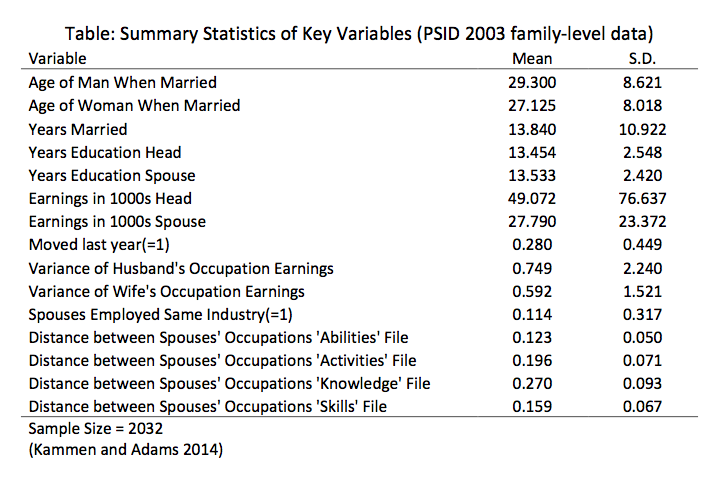
\includegraphics[width=\textwidth, height=0.85\textheight]{table.png}
\end{frame}
 
\section{Methodology}
\begin{frame}
\frametitle{Methodology}
\mysphere human capital model\\
\mysphere Occupation similarity level: O*Net Content Model\\
\mysphere Occupation similarity and mobility
\end{frame}
 
\end{document}